\section{Experiments}
In section~\ref{subsec:poam} and \ref{subsec:7racfm}, we assume Euclidean configuration spaces $Q$ and focus on examples with fixed initial and final points $q_i, q_f \in Q$, therefore we use the via-point affine curve model from VMP~\cite{zhou2019learning}: 
\begin{equation}
\label{eq:acme}
    q(\tau; w) = (1-\tau)q_i + \tau q_f + w \phi(\tau),
\end{equation}
where $\phi_i(\tau) = \tau(1-\tau) \ b_i^G(\tau) / \sum_{j} b_j^G(\tau)$ (it is trivial to show the linear independence of $\phi_i$; see Proposition~\ref{prop:prop3}).
To give hard constraints of initial and final points to $q(\tau; w)$, we multiply $\tau(1-\tau)$ to the original basis term from \cite{zhou2019learning}. 

One might wonder whether it is always necessary to design parametric curve models in an environment-specific manner. We note that the parametric curve model (\ref{eq:affinemodel}), with the choice of \(\psi(\tau)=0\) and $\phi_i(\tau)=\ b_i^G(\tau) / \sum_{j} b_j^G(\tau)$, is sufficiently expressive to model any smooth, arbitrary complex trajectory with a sufficiently large \(B\). Thus, no special modeling is required if we do not enforce any constraints on the curve.
If we have desired constraints, we can, in some cases, design suitable parametric models that guarantee these constraints are satisfied. For example, if we want \(q(\tau)\) to pass through \((\tau_i, q_i)\) and \((\tau_i, \dot{q}_i)\) for \(i = 1, \ldots, N\), we can design \(\psi(\tau)\) to be the lowest-order polynomial that satisfies \((\tau_i, q_i)\) and \((\tau_i, \dot{q}_i)\) for all \(i\), and set \(\phi(\tau) = \Pi_i (\tau - \tau_i)^2 b^G_j(\tau)/\sum_j b^G_j(\tau)\).

We compare MMP++, IMMP++, and VMP~\cite{zhou2019learning}. We utilize Gaussian Mixture Models (GMMs) to fit latent density models for MMP++ and IMMP++ unless otherwise specified. While the distribution of $w$ is assumed to be Gaussian in vanilla VMP, it has limitations in capturing multi-modal distributions. To ensure a fair comparison, we also implement VMP with GMM. When sampling new trajectories from fitted distributions, we reject the samples with likelihood values lower than the threshold value $\eta$ -- where $\eta$ is set to be the minimum value among the likelihood values of the training trajectories. 

In section~\ref{subsec:SE3}, we consider the position-orientation space 
\[
    {\rm SE}(3) := \{(p, R) \: | \: p \in \mathbb{R}^{3}, R \in {\rm SO}(3)\},
\]
where ${\rm SO}(3) := \{R \in \mathbb{R}^{3\times 3}\: | \: R^TR = I, \det(R)=1\}$ is the group of rotation matrices; $p$ and $R$ denote the position and orientation, respectively. In the position space $\mathbb{R}^{3}$, we use the affine curve model $p(\tau; w)$ in (\ref{eq:acme}). In the orientation space ${\rm SO}(3)$, we use a tailored parametric curve model $R(\tau; w)$, of which details will be given later in the corresponding section. 
In comparison to the MMP with discrete-time trajectory representations in~\cite{lee2023equivariant}, we show that our MMP++ enables additional modulations of initial and final positions and orientations. 

\subsection{Planar Obstacle-Avoiding Motions}
\label{subsec:poam}
\begin{figure}[!t]
    \centering
    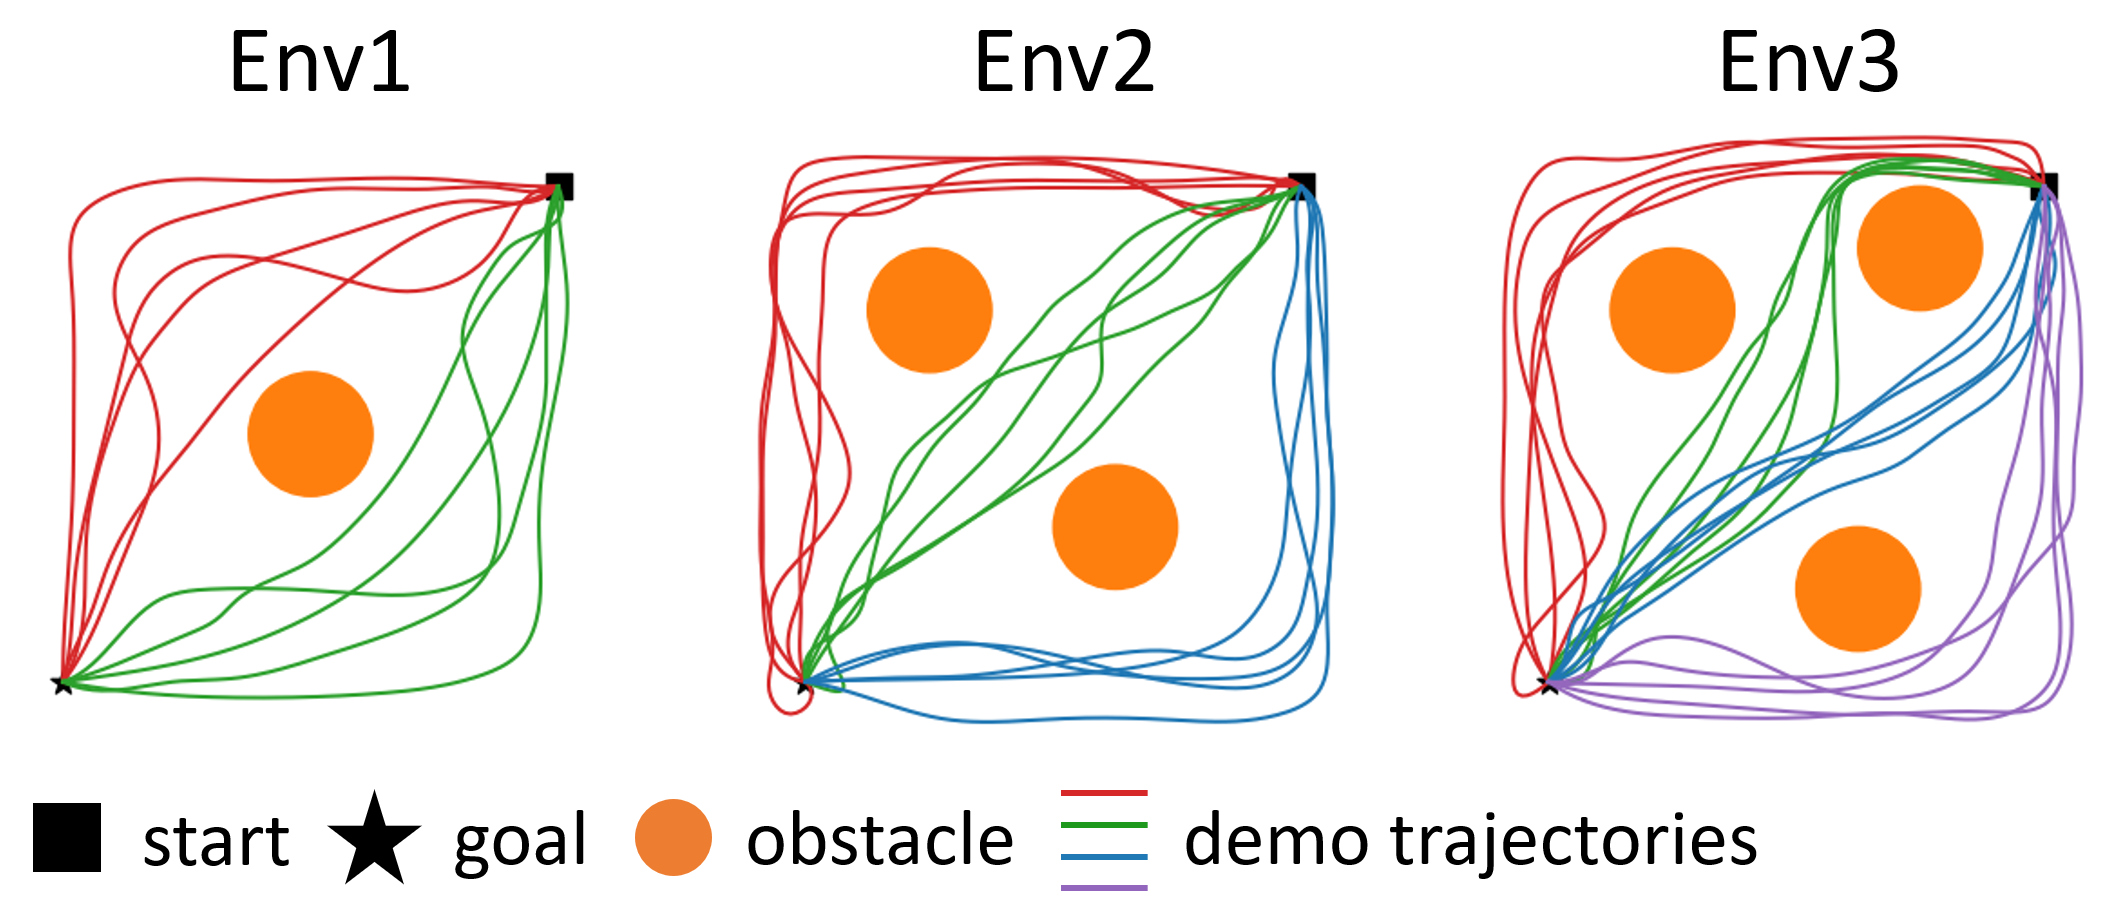
\includegraphics[width=\linewidth]{figure/expsetting.png}
    \caption{Three environments with training demonstration trajectories.}
    \label{fig:expsetting}
    \vspace{-5pt}
\end{figure}

We consider three different environments with different numbers of obstacles and obstacle-avoiding trajectories; see Env1, Env2, and Env3 in Fig.~\ref{fig:expsetting}. 
The number of total training trajectories for each environment setting is 10, 15, and 20, respectively. 
The number of basis $B=20$ for $\phi(\tau)$. In MMP++ and IMMP++. 
The latent space dimension is search among 2, 3, 4, and 5
The number of GMM components is set to be 2, 3, and 4 for Env1, Env2, and Env3, respectively.
A generated trajectory is considered successful if it does not collide with the obstacles. 

As shown in Table~\ref{tab:toy} and Fig.~\ref{fig:exp1}, the IMMP++ performs the best compared to the other methods. 
Sometimes, MMP++ fails significantly because GMM fits wrong clusters due to the geometric distortions in the latent coordinate spaces; see Fig.~\ref{fig:intro} for example latent spaces of MMP+ and IMMP++.

\begin{table}[!t]
    \centering
    \caption{Averages and standard deviations of the success rates with 5 times run with different random seeds; the higher the better. The best results are marked in bold.}
    \label{tab:toy}
    \begin{tabular}{l|ccc}
                         & Env1 & Env2 & Env3 \\ \hline
        VMP (Gaussian)   & 76.42 $\pm$ 1.34 & 65.76 $\pm$ 1.60 & 38.24 $\pm$ 1.18  \\
        VMP (GMM)        & 97.12 $\pm$ 0.51 & 97.52 $\pm$ 0.30 & 98.14 $\pm$ 0.24  \\
        MMP++ (ours)     & 99.48 $\pm$ 0.38 & 88.58 $\pm$ 0.60 & 97.76 $\pm$ 1.46 \\
        IMMP++ (ours)    & {\bf 100.00 $\pm$ 0.00} & {\bf 99.90 $\pm$ 0.12} & {\bf 99.22 $\pm$ 0.19}
    \end{tabular}
\end{table}

\begin{figure}[!t]
    \centering
    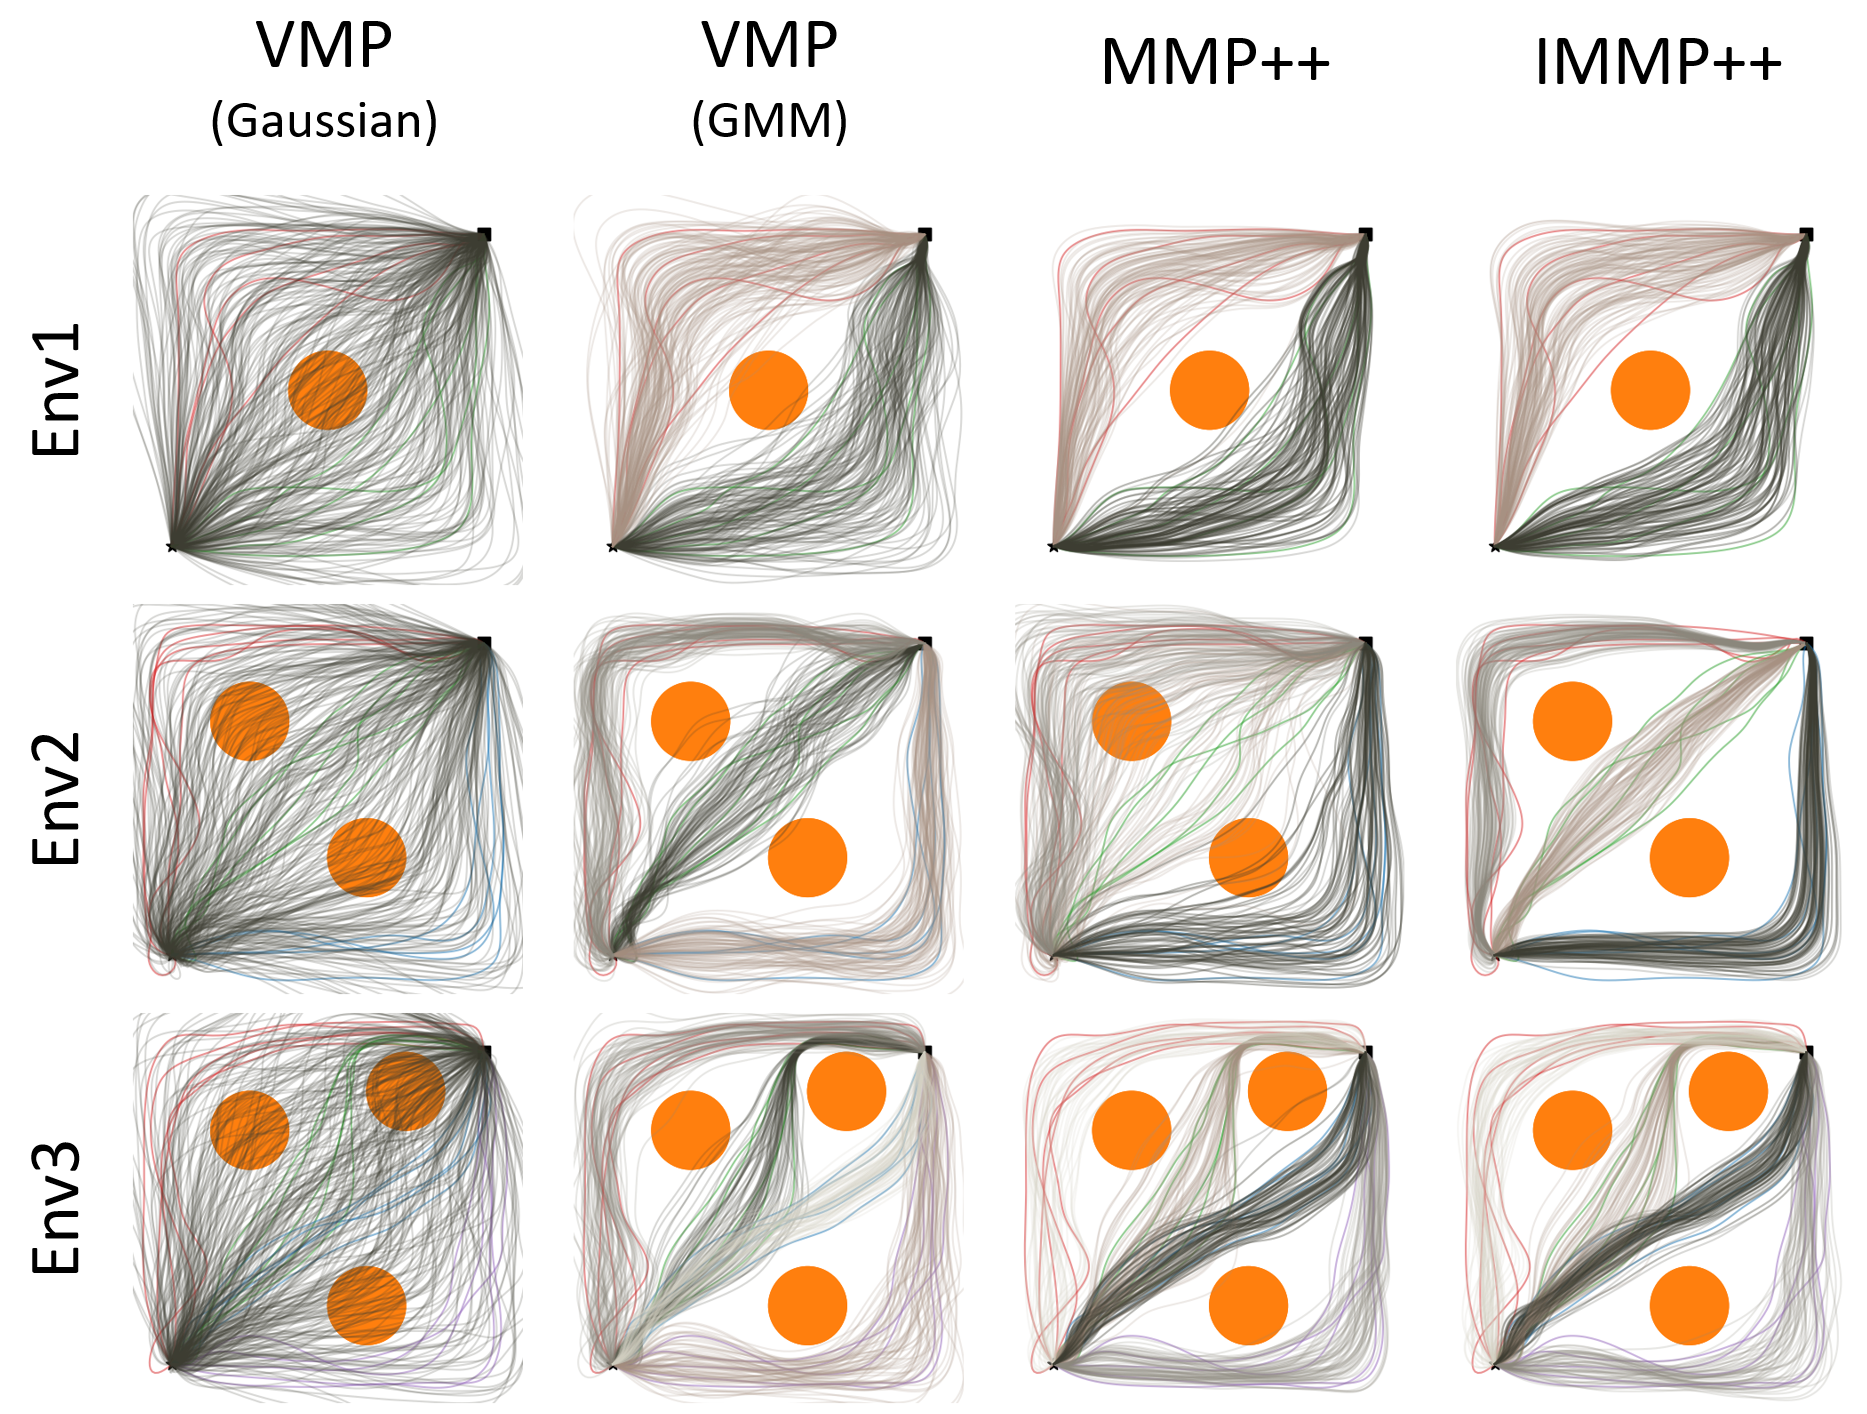
\includegraphics[width=1\linewidth]{figure/toy_results.png}
    \caption{Trajectories generated by trained models. The GMM component numbers are 2, 3, and 4 for Env1, Env2, and Env3, respectively (samples from the same GMM component are assigned the same color).} 
    \label{fig:exp1}
    \vspace{-5pt}
\end{figure}

\subsection{7-DoF Robot Arm Collision-Free Motions}
\label{subsec:7racfm}
\begin{figure*}[!t]
    \centering
    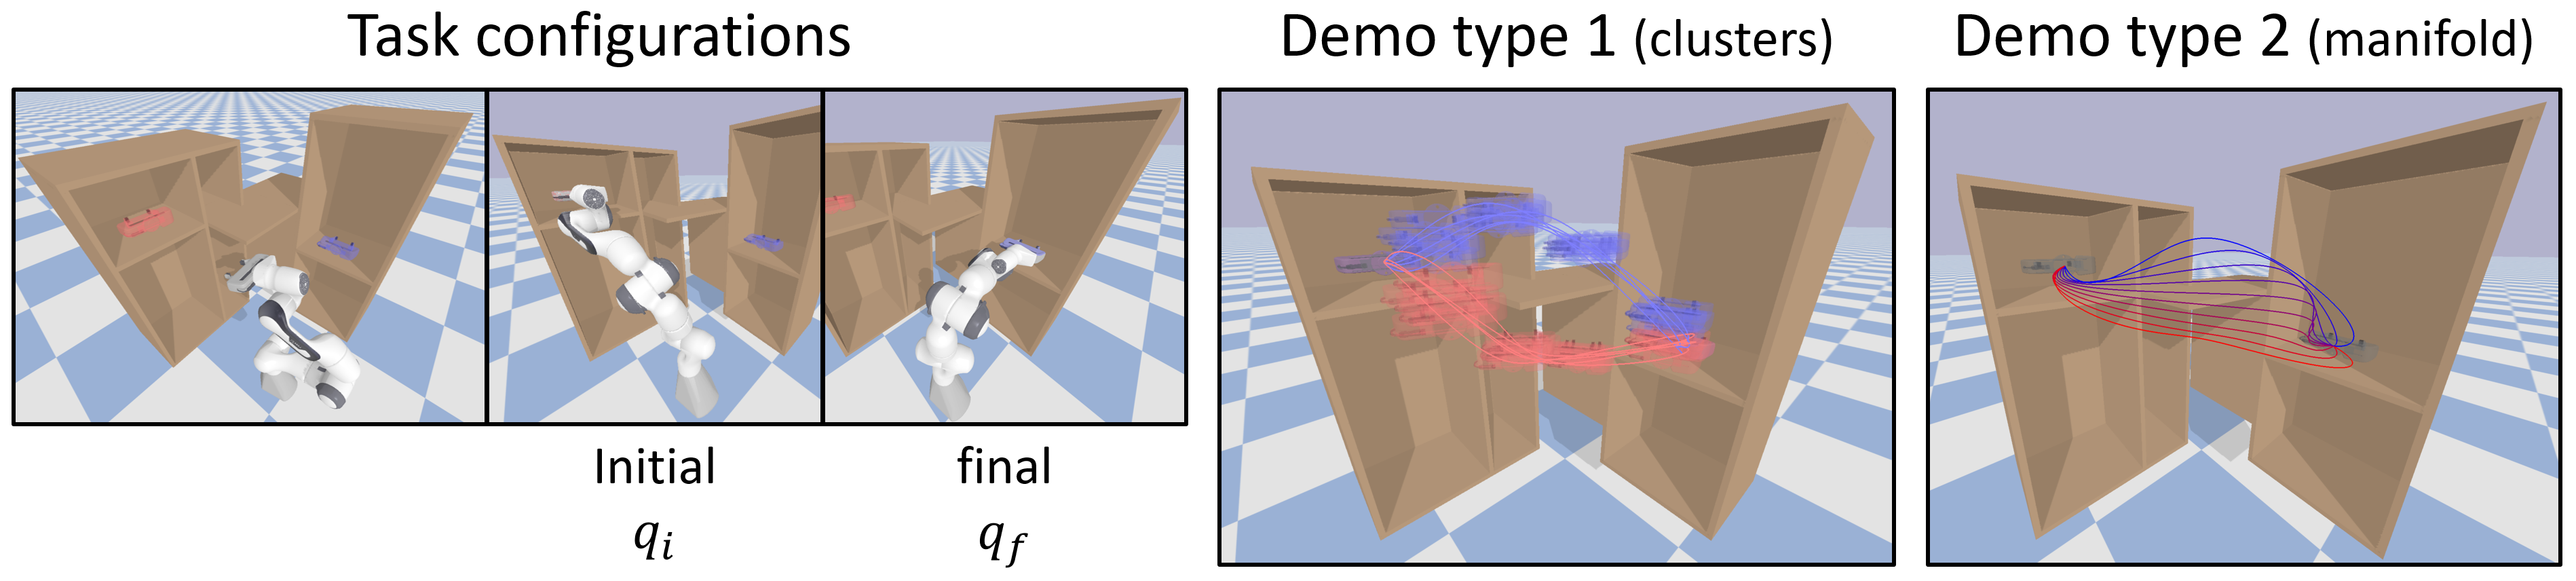
\includegraphics[width=0.9\linewidth]{figure/robot_exp.png}
    \caption{{\it Left}: A 7-DoF robot arm needs to move from the joint configuration $q_i$ to $q_f$ without colliding to the environment. {\it Right}: Two types of demonstration trajectories, where 7-dimensional joint space trajectories are given as demonstration data (only the end-effector's SE(3) or $\mathbb{R}^{3}$ trajectories are visualized). In demo type 1, two clusters of trajectories are given, and, in demo type 2, a one-dimensional manifold of trajectories is provided.} 
    \label{fig:robot_exp}
    \vspace{-5pt}
\end{figure*}

In this section, we consider collision-free point-to-point motions of a 7-DoF Franka Emika Panda robot arm in 
an environment shown in Fig.~\ref{fig:robot_exp} ({\it Left}). Two types of demonstration trajectories are given, each with 10 joint space trajectories -- in Fig.~\ref{fig:robot_exp} ({\it Right}), SE(3) and $\mathbb{R}^{3}$ forward kinematics results of them are visualized for simplicity --, where the initial and final configurations are identical as $q_i$ and $q_f$ in Fig.~\ref{fig:robot_exp} ({\it Left}). 
In the demo type 1, there are two clusters of trajectories, whereas in the demo type 2 a set of trajectories forms an 1-dimensional manifold, a trajectory manifold embedded in the trajectory space. The number of basis $B=20$ for $\phi(\tau)$. In MMP++ and IMMP++, the latent space dimensions are 2. The number of GMM components is 2. Exceptionally, for MMP++ and IMMP++ applied to the demo type 2, we use the Kernel Density Estimator (KDE) instead of the GMM (we will provide the reason later).

Table~\ref{tab:robot} shows the averages and standard deviations of the success rates. Overall, MMP++ and IMMP++ show the best performances.
In particular, VMPs show far inferior results than our manifold-based methods given a manifold of demonstrations in the demo type 2. This is because neither Gaussian nor GMM models are suitable for capturing the continuous manifold structure of the density's support.
Fig.~\ref{fig:robot_results} shows the two-dimensional latent spaces of the manifold-based methods. 
For demo type 1, the distance between clusters in the latent space of IMMP+ is greater than that in the latent space of MMP++. 
Even though MMP++ successfully captures correct clusters in this particular dataset, for more complex datasets, it is more likely to fail in capturing correct clustering structures.

For demo type 2, we note that two-dimensional encoded latent points form an one-dimensional manifold; 
it should be considered as a single connected manifold component. 
Given this manifold support, we found that it is sub-optimal to use the GMM for fitting a distribution. 
Hence, we use a non-parametric method, KDE, that can more accurately estimate our latent space density function:
\begin{equation}
\label{eq:KDE_density}
    p(z) = \frac{1}{N}\sum_{i=1}^{N}\frac{1}{2\pi|H_i|^{1/2}} \exp(- \frac{(z-z_i)^T H_i^{-1} (z-z_i)}{2}),
\end{equation}
where $\{z_i\}_{i=1}^{N}$ is the set of encoded latent points and $H_i,i=1,\ldots,N$ are positive-definite matrices. 
Let $K(z_i, z_k) = \exp(-\|z_i-z_k\|^2/h)$; for this example, we construct $H_i=\Sigma_i^2$ where
\begin{equation}
    \Sigma_i = \frac{\sum_{k=1}^{N} K(z_i, z_k) (z_i - z_k) (z_i - z_k)^T}{\sum_{k=1}^{N} K(z_i, z_k)}.
\end{equation}

One may ask if using such a non-parametric method in the curve parameter space ${\cal W}$ of VMP directly can lead to a better performance than using GMM. Unfortunately, this is challenging due to the high-dimensional nature of ${\cal W}$. It is worth noting that this approach is feasible in MMP++ and IMMP++ because we utilize sufficiently low-dimensional latent spaces.

\begin{table}[!t]
    \centering
    \caption{Averages and standard deviations of the success rates with 5 times run with different random seeds; the higher the better. The best results are marked in bold.}
    \label{tab:robot}
    \begin{tabular}{c|cccc}
        Demo & \begin{tabular}{c} VMP \\ (Gaussian) \end{tabular} &  \begin{tabular}{c} VMP \\ (GMM)\end{tabular} & \begin{tabular}{c} MMP++ \\ (ours) \end{tabular} & \begin{tabular}{c} IMMP++ \\ (ours) \end{tabular} \\ \hline
         type 1 & 46.1 $\pm$ 4.37 & 97.1 $\pm$ 1.66 & 98.6 $\pm$ 0.20 & {\bf 99.5 $\pm$ 0.77} \\
         type 2 & 79.4 $\pm$ 2.94 & 83.0 $\pm$ 3.78 & {\bf 99.3 $\pm$ 0.68}  & 98.2 $\pm$ 0.68  \\
    \end{tabular}
    \vspace{-5pt}
\end{table}

\begin{figure}[!t]
    \centering
    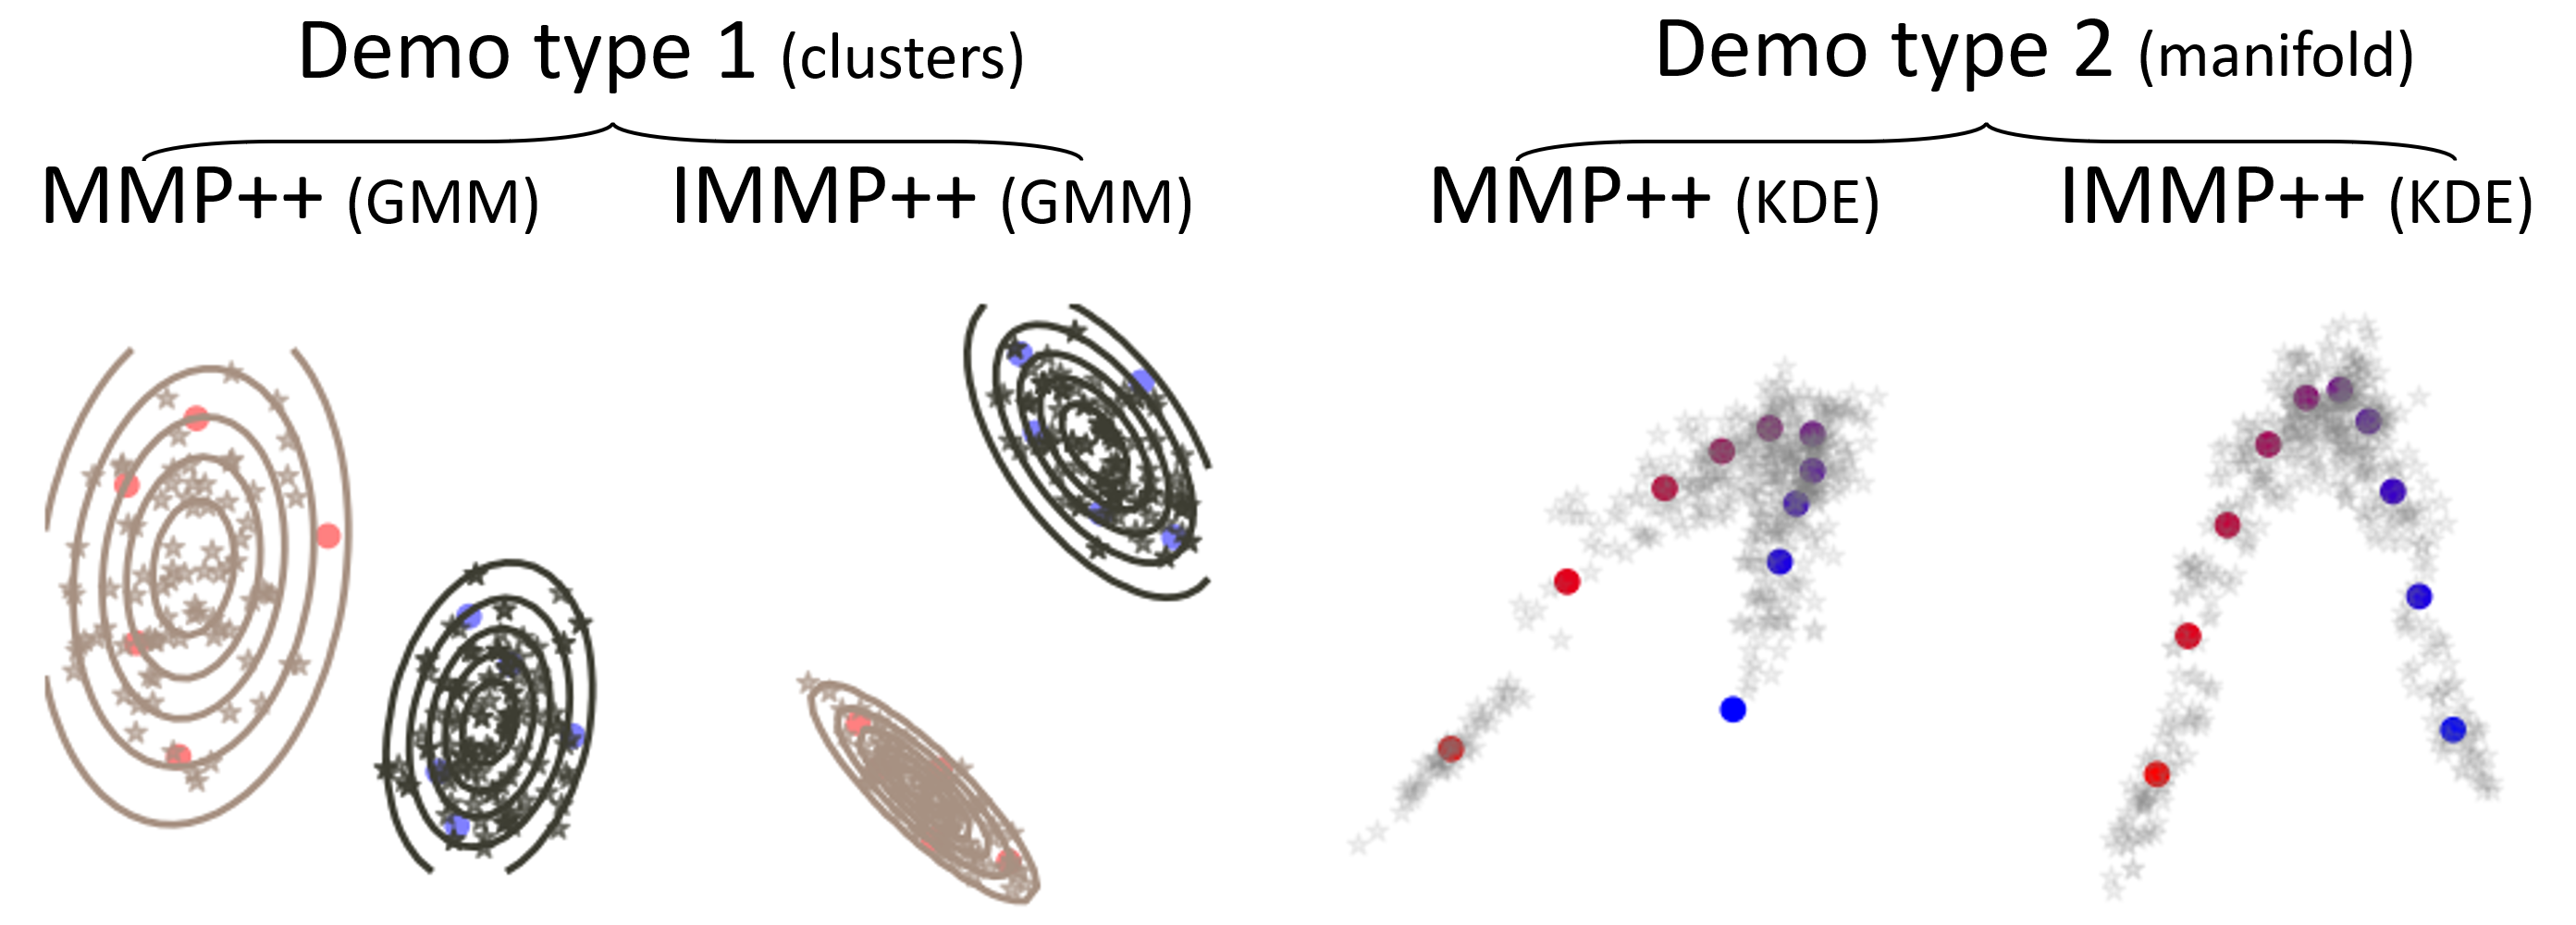
\includegraphics[width=1\linewidth]{figure/robot_results.png}
    \caption{The two-dimensional latent spaces of our manifold-based methods (MMP++ and IMMP++) are illustrated (circular points are encoded points and star-shaped points are generated samples). Demonstration trajectories in Fig.~\ref{fig:robot_exp} ({\it Right}) are encoded into these latent spaces, with colors indicating correspondence (e.g., a red trajectory is encoded into a red point).} 
    \label{fig:robot_results}
    \vspace{-5pt}
\end{figure}

Next, we qualitatively show the latent coordinates and via-points modulation results of IMMP++ trained with the demo type 2 (manifold) in Fig.~\ref{fig:manifol_results}. Note that we have the model $q(\tau;f(z))=(1-\tau)q_i + \tau q_f + f(z)\phi(\tau)$ with the trained decoder function $w=f(z)$, where modulations in the latent coordinate value $z$ and the initial and final configurations $q_i$ and $q_f$ lead to corresponding changes in the resulting trajectory $q(\tau)$. In Fig.~\ref{fig:manifol_results} ({\it Upper}), a continuous change in the latent value $z$ leads to a smooth transition of $q(\tau)$ from an upward-moving path to a downward-moving path. As shown in Fig.~\ref{fig:manifol_results} ({\it Middle} and {\it Lower}), continuous changes in $q_i$ and $q_f$ induce smooth changes of $q(\tau)$. 

\begin{figure*}[!t]
    \centering
    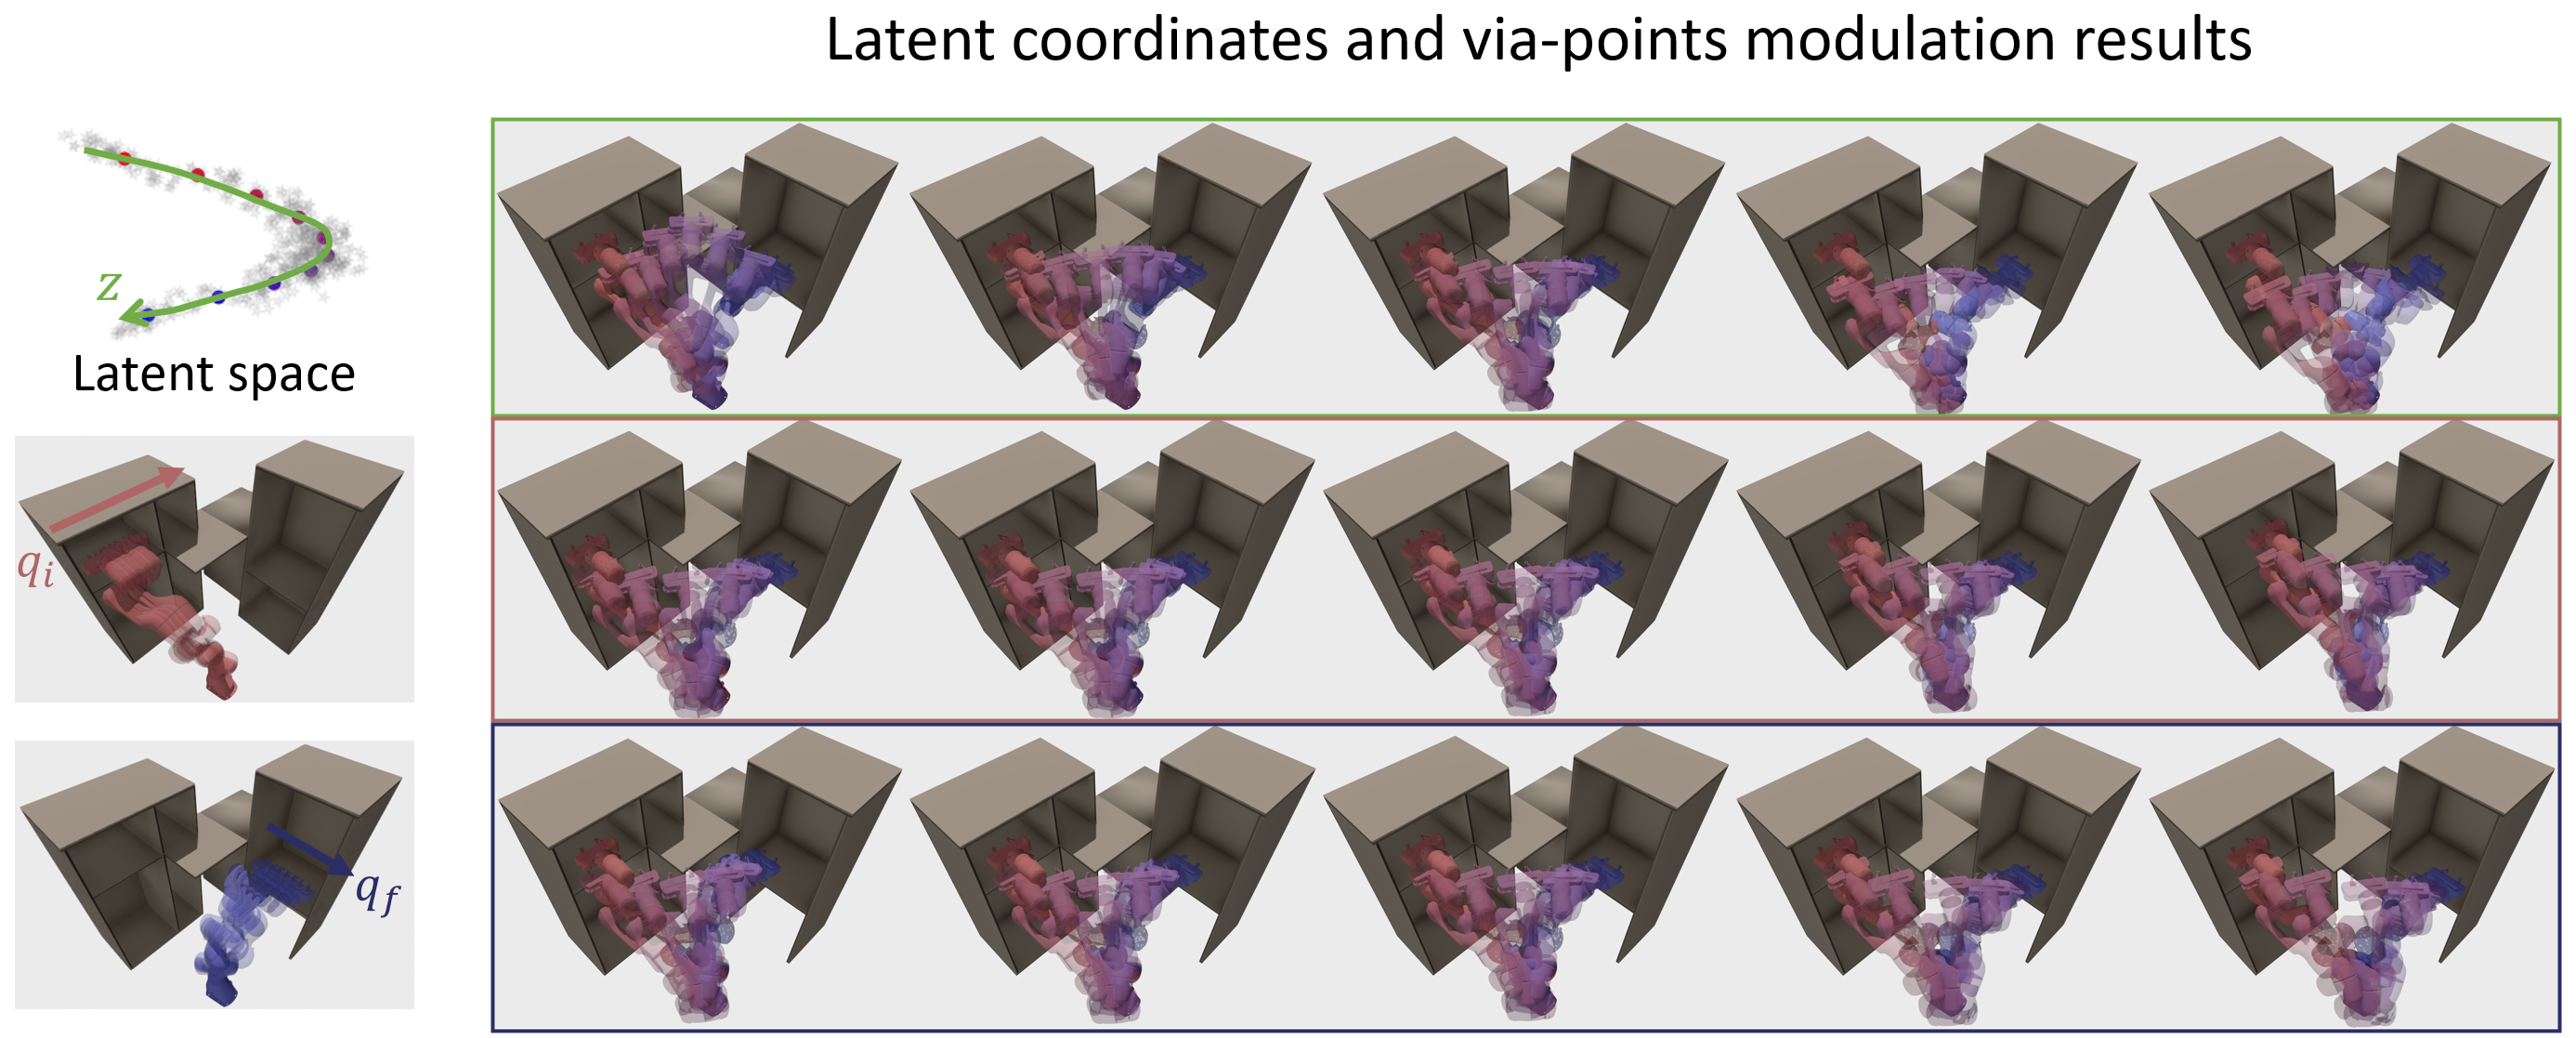
\includegraphics[width=0.85\textwidth]{figure/manifol_results.png}
    \caption{Modulations of latent coordinates $z$ and initial and final configurations $q_i$ and $q_f$ in IMMP++ $q(\tau;f(z))=(1-\tau)q_i + \tau q_f + f(z)\phi(\tau)$. {\it Upper}: A continuous change in $z$ results in a smooth transition of $q(\tau)$. {\it Middle}: Changes in $q_i$ induce smooth transitions of $q(\tau)$. {\it Lower}: Changes in $q_f$ induce smooth transitions of $q(\tau)$.} 
    \label{fig:manifol_results}
    \vspace{-5pt}
\end{figure*}

Lastly, we show the adaptability of our primitive models in the presence of unseen constraints and propose a novel online iterative re-planning algorithm. We will consider $(z, \tau)$ as a state. Let $T$ be a total time length. First of all, suppose we do not have additional unseen constraints. We start with a random initial $z \sim p(z)$ and $\tau=0$. Then, as the time $\delta t$ passes, $z$ remains constant and $\tau$ is updated to $\min(\tau + \delta t/T, 1)$. At each time step, we use $q(\tau; f(z))$ as a desired joint configuration and run a position controller with the control frequency $f_c$. This procedure is just a position tracking control given an initially-planned trajectory $q(\tau; f(z))$. 

Now, consider a situation where an obstacle that blocks the initially-planned trajectory appears and moves as the time flows as shown in Fig.~\ref{fig:MPC}. We assume constraints are given as inequality equations $C(q) \leq 0$ in the configuration space ${\cal Q}$, which can change dynamically in time. Suppose our current state is $(z,\tau)$. We set a time window $t_w$ and if $C(q(\bar{\tau}; f(z)) > 0$ for some $\tau < \bar{\tau} < \tau + t_w/T$, we re-plan the trajectory, i.e., update and find a new desired state $(z',\tau')$, with the re-planning frequency $f_p < f_c$. 
Given a new desired state $(z', \tau')$, we will update $z \xleftarrow{} z + k (z'-z)$ and $\tau \xleftarrow{} \tau + k (\tau'-\tau)$ with positive gain $k$ at control frequency $f_c$ for time $1/f_p$, and then decide whether we will re-plan $(z,\tau)$ again or not. Considering this update rule, in the re-planning step, we find $(z',\tau')$ by solving the following optimization problem:
\begin{align}
\label{eq:mpc_sa}
    \min_{(z', \tau')}  \: \|z - &z'\|^2  + \alpha \|\tau - \tau'\|^2 \\
    {\rm such} \: {\rm that} \:\: & {\rm (1)} \:\: C(q(\bar{\tau}'; f(z')) \leq 0 \nonumber \\ 
    & \:\:\:\:\:\:\:\:\: \tau' < \bar{\tau}' < \tau' + t_w/T \nonumber \\
    & {\rm (2)} \:\: \log p(z') \geq \epsilon \nonumber \\ 
    & {\rm (3)} \:\:  C(q(\tau_{\eta}; f(z_\eta)) \leq 0 \:\: \& \:\: \log p(z_\eta) \geq \epsilon \nonumber \\ 
    & \:\:\:\:\:\:\:\:\: z_\eta=\eta z + (1-\eta) z' \nonumber \\ 
    & \:\:\:\:\:\:\:\:\: \tau_\eta = \eta \tau + (1-\eta)\tau' \nonumber \\
    & \:\:\:\:\:\:\:\:\: \eta \in [0,1] \nonumber \\
    & {\rm (4)} \:\: \tau' \in [\tau - \delta, \tau] \nonumber, 
\end{align}

where the weight $\alpha > 0$ is set to be big enough to prioritize updating $z$. (1) enforces the planned trajectory from $(z',\tau')$ to satisfy the constraints for time $t_w$, (2) prevents $z'$ from being out-of-distribution in the latent space ($\epsilon$ is the log probability density threshold; we set it to be the minimum value among the log likelihood values of the training data), (3) guarantees the linear path connecting the current and next states from $(z,\tau)$ to $(z',\tau')$ satisfies the constraints and lies within the in-distribution region in the latent space, and (4) allows $\tau' \in [\tau-\delta, \tau]$ -- where $\delta$ is the max travel-back time -- in case no feasible $z'$ exists when $\tau' = \tau$. 
A pseudocode for our online iterative re-planning algorithm is provided in Algorithm~\ref{alg:OIR}.
\begin{algorithm}[!t]
\caption{Online Iterative Trajectory Re-planning with MMP++}
\label{alg:OIR}
\KwIn{MMP++ decoder $w=f(z)$, parametric curve $q(\tau; w)$, latent density $p(z)$, inequality constraint $C(q)\leq 0$, time window $t_w$, total time length $T$, gain $k>0$, control frequency $f_c$, re-planning frequency $f_p$, and optimization solver SOLVE (\ref{eq:mpc_sa}) }
{\bf Initialization:} $z \sim p(z)$, $\tau=0$, $c_v={\rm False}$ \\
\While{True}{
Once every $1/f_p$ seconds: \\
  \eIf{$C(q(\bar{\tau}; f(z))) > 0$ for some $\bar{\tau} \in [\tau, \min(\tau + t_w/T, 1)]$}{
    $(z_g, \tau_g) \xleftarrow[]{}$ SOLVE (\ref{eq:mpc_sa}) \\
    $c_v={\rm True}$
  }{
    $c_v={\rm False}$
  }
Once every $1/f_c$ seconds: \\
  \eIf{$c_v$}{
    $z \xleftarrow[]{} z + k(z_g - z)$ \\ 
    $\tau \xleftarrow[]{} \tau + k(\tau_g - \tau)$
  }{
    $z \xleftarrow{} z$ \\
    $\tau \xleftarrow[]{} \min(\tau + 1/(f_cT), 1)$
  }
Position control input: $q(\tau; f(z))$
}
\end{algorithm}

% \begin{algorithm}
%   \caption{Online iterative re-planning with MMP++}
%   \begin{algorithmic}[1]
%     \REQUIRE Decoder $w=f(z)$, parametric curve $q(\tau; w)$, latent density $p(z)$, constraint $C(q)\leq 0$, weight $\alpha>0$, max travel-back time $\delta>0$, log density threshold $\epsilon$, time window $t_w$, total time length $T$, control frequency $f_c$, and re-planning frequency $f_p$
%     \STATE \textbf{Initialization} $z \sim p(z)$, $\tau=0$, ${\rm collision}=0$
%     \WHILE{True}
%     \IF
%     \STATE If ${\rm collision}==0$:
%       \STATE $\tau \xleftarrow{} \min(\tau + \frac{1}{f_c T}, 1)$, $z \xleftarrow{} z$
%       \STATE Compute position control input : $q_d = q(\tau; f(z))$
%     \ENDWHILE
%   \end{algorithmic}
% \end{algorithm}

We can efficiently solve the optimization (\ref{eq:mpc_sa}) thanks to the low-dimensionality of the optimization variable $(z', \tau')$. 
In the example in Fig.~\ref{fig:MPC}, we use IMMP++ trained with the demo type 2 (manifold). As visualized in Fig.~\ref{fig:MPC} ({\it Upper-Right}), given a dynamically changing constraint (i.e., moving spherical obstacle), the robot iteratively re-plans its trajectory whenever it is predicted to collide with the obstacle within the time interval $t_w$. A gradient-free sampling-based optimization approach is fast enough and shows a successful online iterative re-planning result. Fig.~\ref{fig:MPC} ({\it Lower}) shows $\|z\|$ and $\tau$ as functions of time, indicating when $(z,\tau)$ is re-planned. It can be confirmed that at around $t=2$ the robot predicted collisions with the obstacle within $t_w=1$ and re-planned $(z, \tau)$ multiple times.

\begin{figure}[!t]
    \centering
    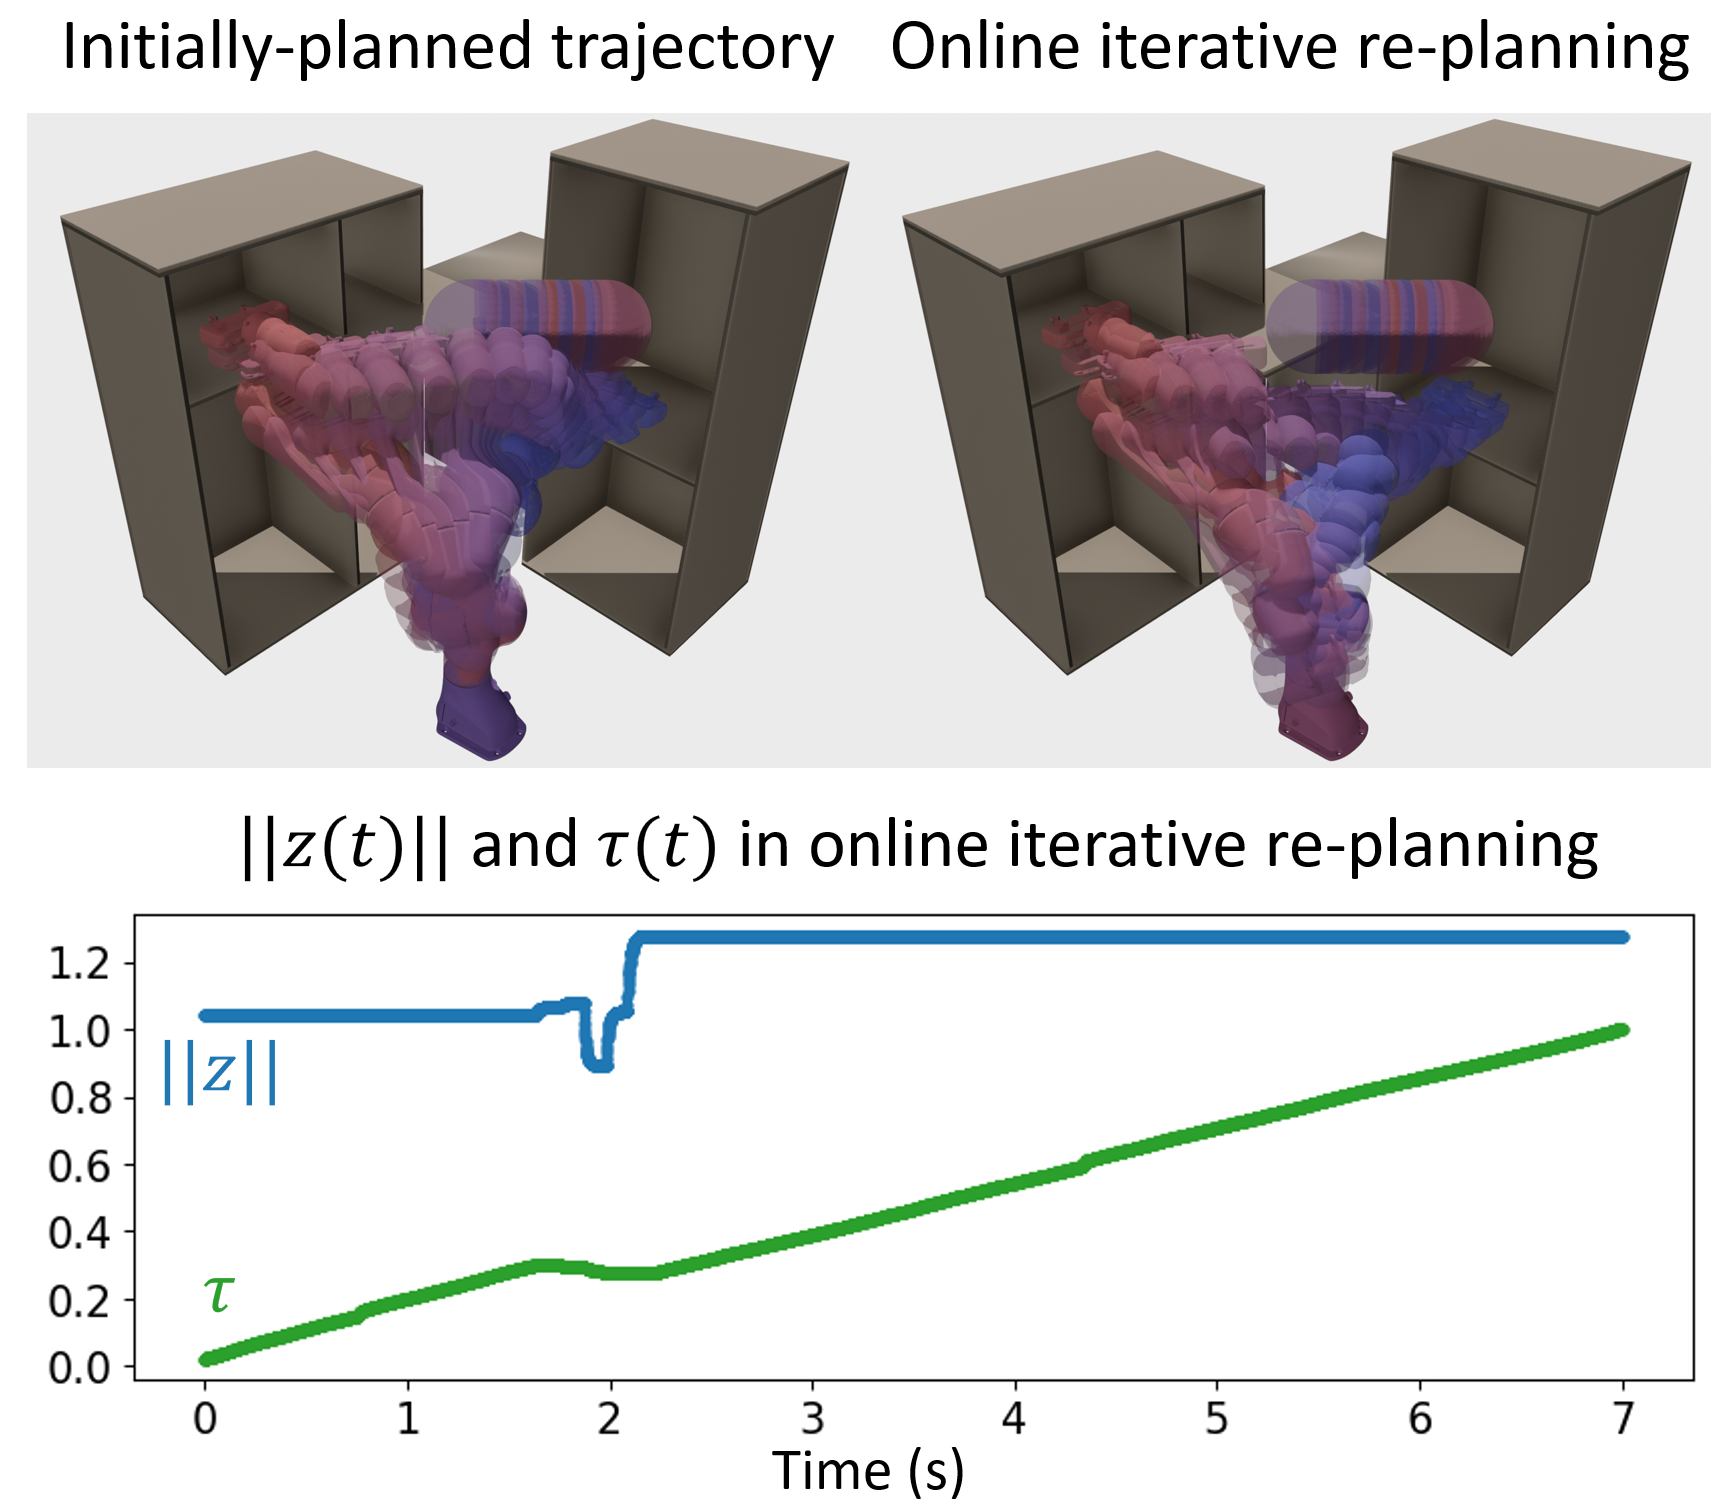
\includegraphics[width=0.9\linewidth]{figure/MPC.png}
    \caption{{\it Upper-Left:} Initially-planned trajectory is blocked by the unseen obstacle during training. {\it Upper-Right:} The robot iteratively re-plans its trajectory whenever it is predicted to collide with the obstacle. {\it Lower:} $\|z\|$ and $\tau$ as functions of time $t$ in online iterative re-planning ({\it Upper-Right}), where $T=5$, $t_w=1$, $f_c=1000$, and $f_p=10$.} 
    \label{fig:MPC}
\end{figure}

\begin{table}[!t]
    \centering
    \small
    \caption{Computation times for planning via RRT-Connect~\cite{kuffner2000rrt} and IMMP++ are measured with three times run. We consider a shelf-only environment, the shelf with one spherical obstacle, and the shelf with two spherical obstacles; see Fig.~\ref{fig:IMMP_vs_RRT}. Computations are performed using an AMD Ryzen 9 5900x 12-Core Processor and an NVIDIA GeForce RTX 3090. All code is implemented in Python.}
    \label{tab:IMMP_vs_RRT}
    \begin{tabular}{l|cc}
    & RRT-connect~\cite{kuffner2000rrt} & IMMP++ (ours) \\ \hline
    Shelf & $1.97 \sim 4.81 \  s$ & $0.006 \pm 0.001 \ s$\\ 
    Shelf + One obstacle & $60.41 \sim 134.36 \ s$ & $0.039 \pm 0.001 \ s$ \\ 
    Shelf + Two obstacles & $45.97 \sim 204.56 \ s$ & $0.077 \pm 0.002 \ s$ \\ 
    \end{tabular}
    % \begin{tabular}{c|ccc}
    %      & Shelf &  \begin{tabular}{c} Shelf \\ + One obstacle \end{tabular} & \begin{tabular}{c} Shelf \\ + Two obstacles \end{tabular} \\ \hline 
    %      RRT-connect~\cite{kuffner2000rrt} & $1.97 \sim 4.81 s$ & $60.41 \sim 134.36 s$ & $45.97 \sim 204.56 s$ \\ 
    %      IMMP (ours) & 
    % \end{tabular}
\end{table}

\begin{figure}[!t]
    \centering
    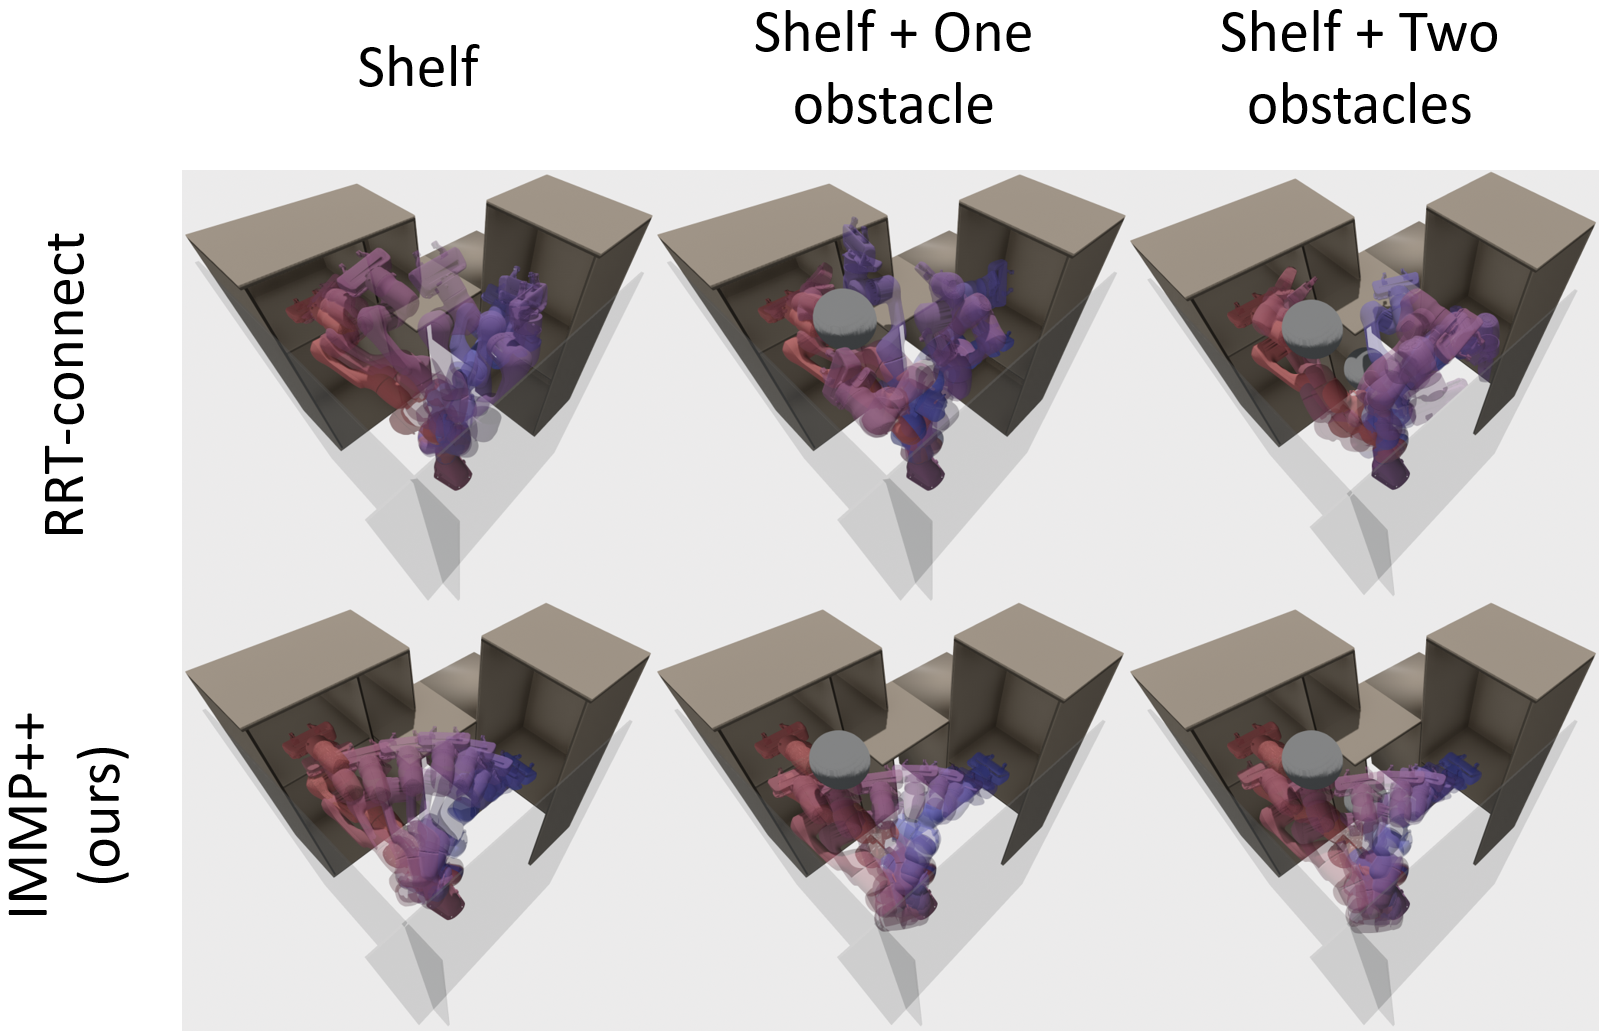
\includegraphics[width=1\linewidth]{figure/IMMP_vs_RRT.jpg}
    \caption{Comparison of collision-free paths planned by RRT-connect~\cite{kuffner2000rrt} and IMMP. Two hypothetical walls, shown as transparent gray, are considered to limit the robot's workspace to the area close to the shelf.}
    \label{fig:IMMP_vs_RRT}
    \vspace{-5pt}
\end{figure}

One can reasonably ask, if we have access to the robot kinematics and the geometry of the environment, what is the advantage of using our method compared to conventional sampling-based collision-free path planning methods, such as RRT variants? Our method offers two important advantages. First, our motion manifold primitives already contain paths that are collision-free for a part of the environment, so only the newly introduced environmental constraints need to be considered during planning. For example, in Fig.~\ref{fig:manifol_results}, the paths in the learned motion manifold do not collide with the shelf. Therefore, when planning within the motion manifold, exact knowledge of the shelf's geometry is unnecessary. While existing sampling-based planning methods require knowledge of all constraints, we only need to consider the new environmental constraints, such as obstacles shown in Fig.~\ref{fig:MPC}.

Second, a more significant advantage is that, while conventional RRTs are typically not fast enough for online dynamic planning, our method is very fast. Table~\ref{tab:IMMP_vs_RRT} shows the computation times for planning using RRT-connect~\cite{kuffner2000rrt} and our IMMP++ in the shelf-only environment and with one and two sphere obstacles, as visualized in Fig.~\ref{fig:IMMP_vs_RRT}. RRT-connect takes several seconds even in the simple shelf-only environment, and the time increases significantly as the complexity of the collision-free configuration space grows due to obstacles. In contrast, our method is relatively much faster. The trajectory sampling in the motion manifold itself takes 0.006 seconds, and the collision checking for obstacles takes only a few milliseconds. Our current implementation is in Python and is sub-optimal. We anticipate that implementing it in a more optimal language would result in even faster performance. Although the RRT algorithm could also be optimized for speed, it is unlikely to become fast enough and suitable for online dynamic planning.

However, these advantages of our algorithm do not come for free. Our method also has limitations. If the learned motion manifold primitives are too small, meaning the generated trajectories are not sufficiently diverse, a collision-free path may not exist on the motion manifold when excessive environmental constraints are introduced. The diversity of the learned motion manifold heavily depends on the diversity of the demonstration data, making the creation of good demonstration trajectories a very important issue.


\subsection{MMP++ for SE(3) Trajectory Data}
\label{subsec:SE3}

In this section, we show how to extend our MMP++ framework to SE(3) trajectory data. 
We will denote the position by $p\in\mathbb{R}^{3}$ and the orientation by $3\times 3 $ rotation matrix $R\in\mathbb{R}^{3\times 3}$. Let $\phi_i(\tau) = \tau(1-\tau) \ b_i^G(\tau) / \sum_{j} b_j^G(\tau)$ for $i=1,\ldots, B$. For the position trajectory, we use the via-point model 
\begin{equation}
p(\tau;w_p) = (1-\tau) p_i + \tau p_f + w_p \phi(\tau),    
\end{equation}
where $w_p \in \mathbb{R}^{3 \times B}$ is the position curve parameter and $p_i,p_f \in \mathbb{R}^{3}$ are initial and final points. 
For the orientation trajectory, we use the following parametric model:
\begin{equation}
\label{eq:rotation_vm}
    R(\tau; w_R) = R_i \exp ( \tau \log (R_i^T R_f))\exp ([w_R\phi(\tau)]),
\end{equation}
where $w_R \in \mathbb{R}^{3 \times B}$ is the orientation curve parameter, $R_i, R_f \in {\rm SO}(3)$ are initial and final orientations, and $\exp(\cdot)$, $\log(\cdot)$ are matrix exponential and logarithm, and 
\[
[(w^1, w^2, w^3)] = \begin{bmatrix}
    0 & -w^3 & w^2 \\ w^3 & 0 & -w^1 \\ -w^2 & w^1 & 0 
\end{bmatrix}
\] is a skew symmetric matrix~\cite{lynch2017modern}.
The orientation via-point model in (\ref{eq:rotation_vm}) is constrained to have the initial and final orientations $R_i$ and $R_f$.

\begin{figure}[!t]
    \centering
    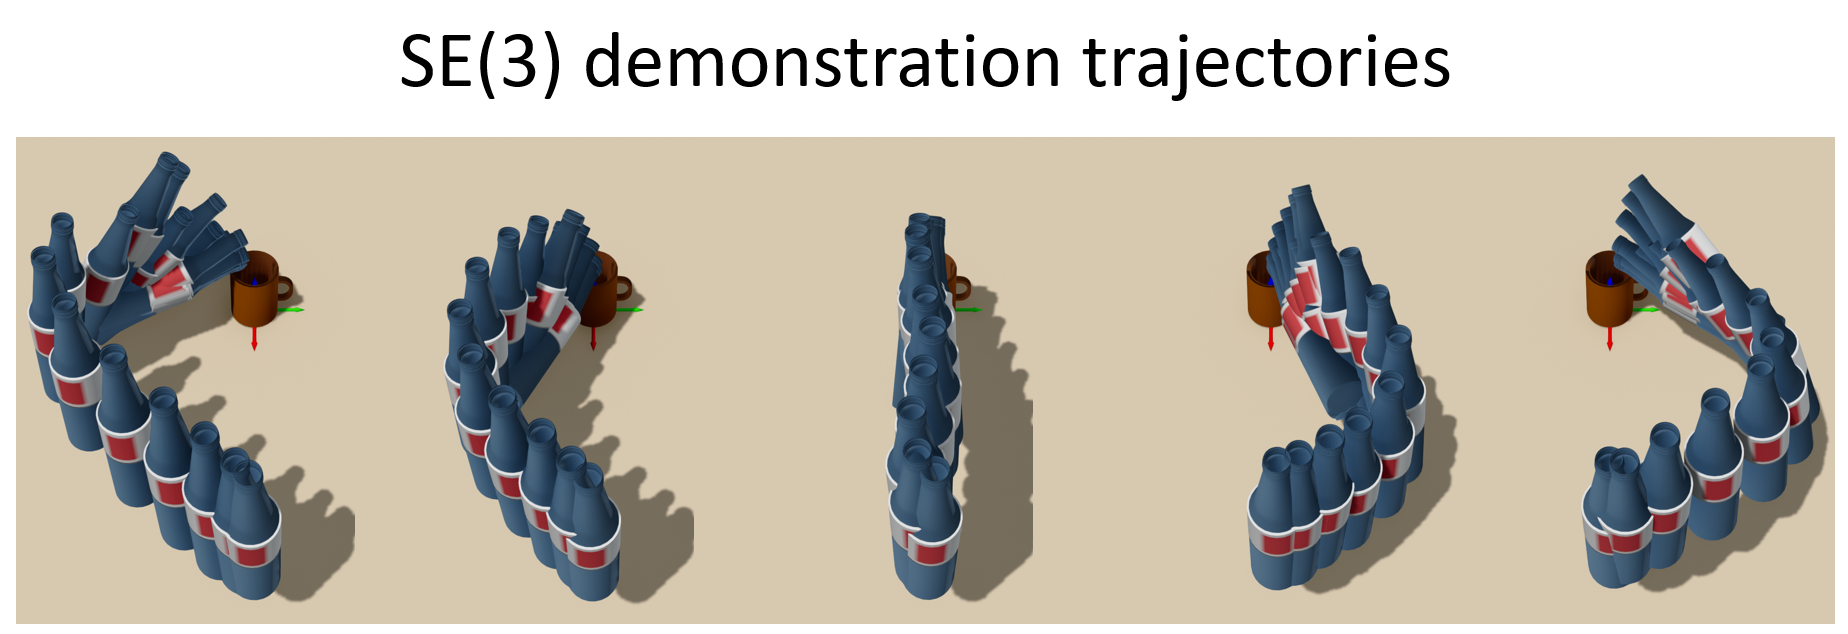
\includegraphics[width=0.85\linewidth]{figure/wp_dataset.png}
    \caption{Water-pouring SE(3) trajectory dataset.} 
    \label{fig:wp_dataset}
    \vspace{-5pt}
\end{figure}

\begin{figure*}[!t]
    \centering
    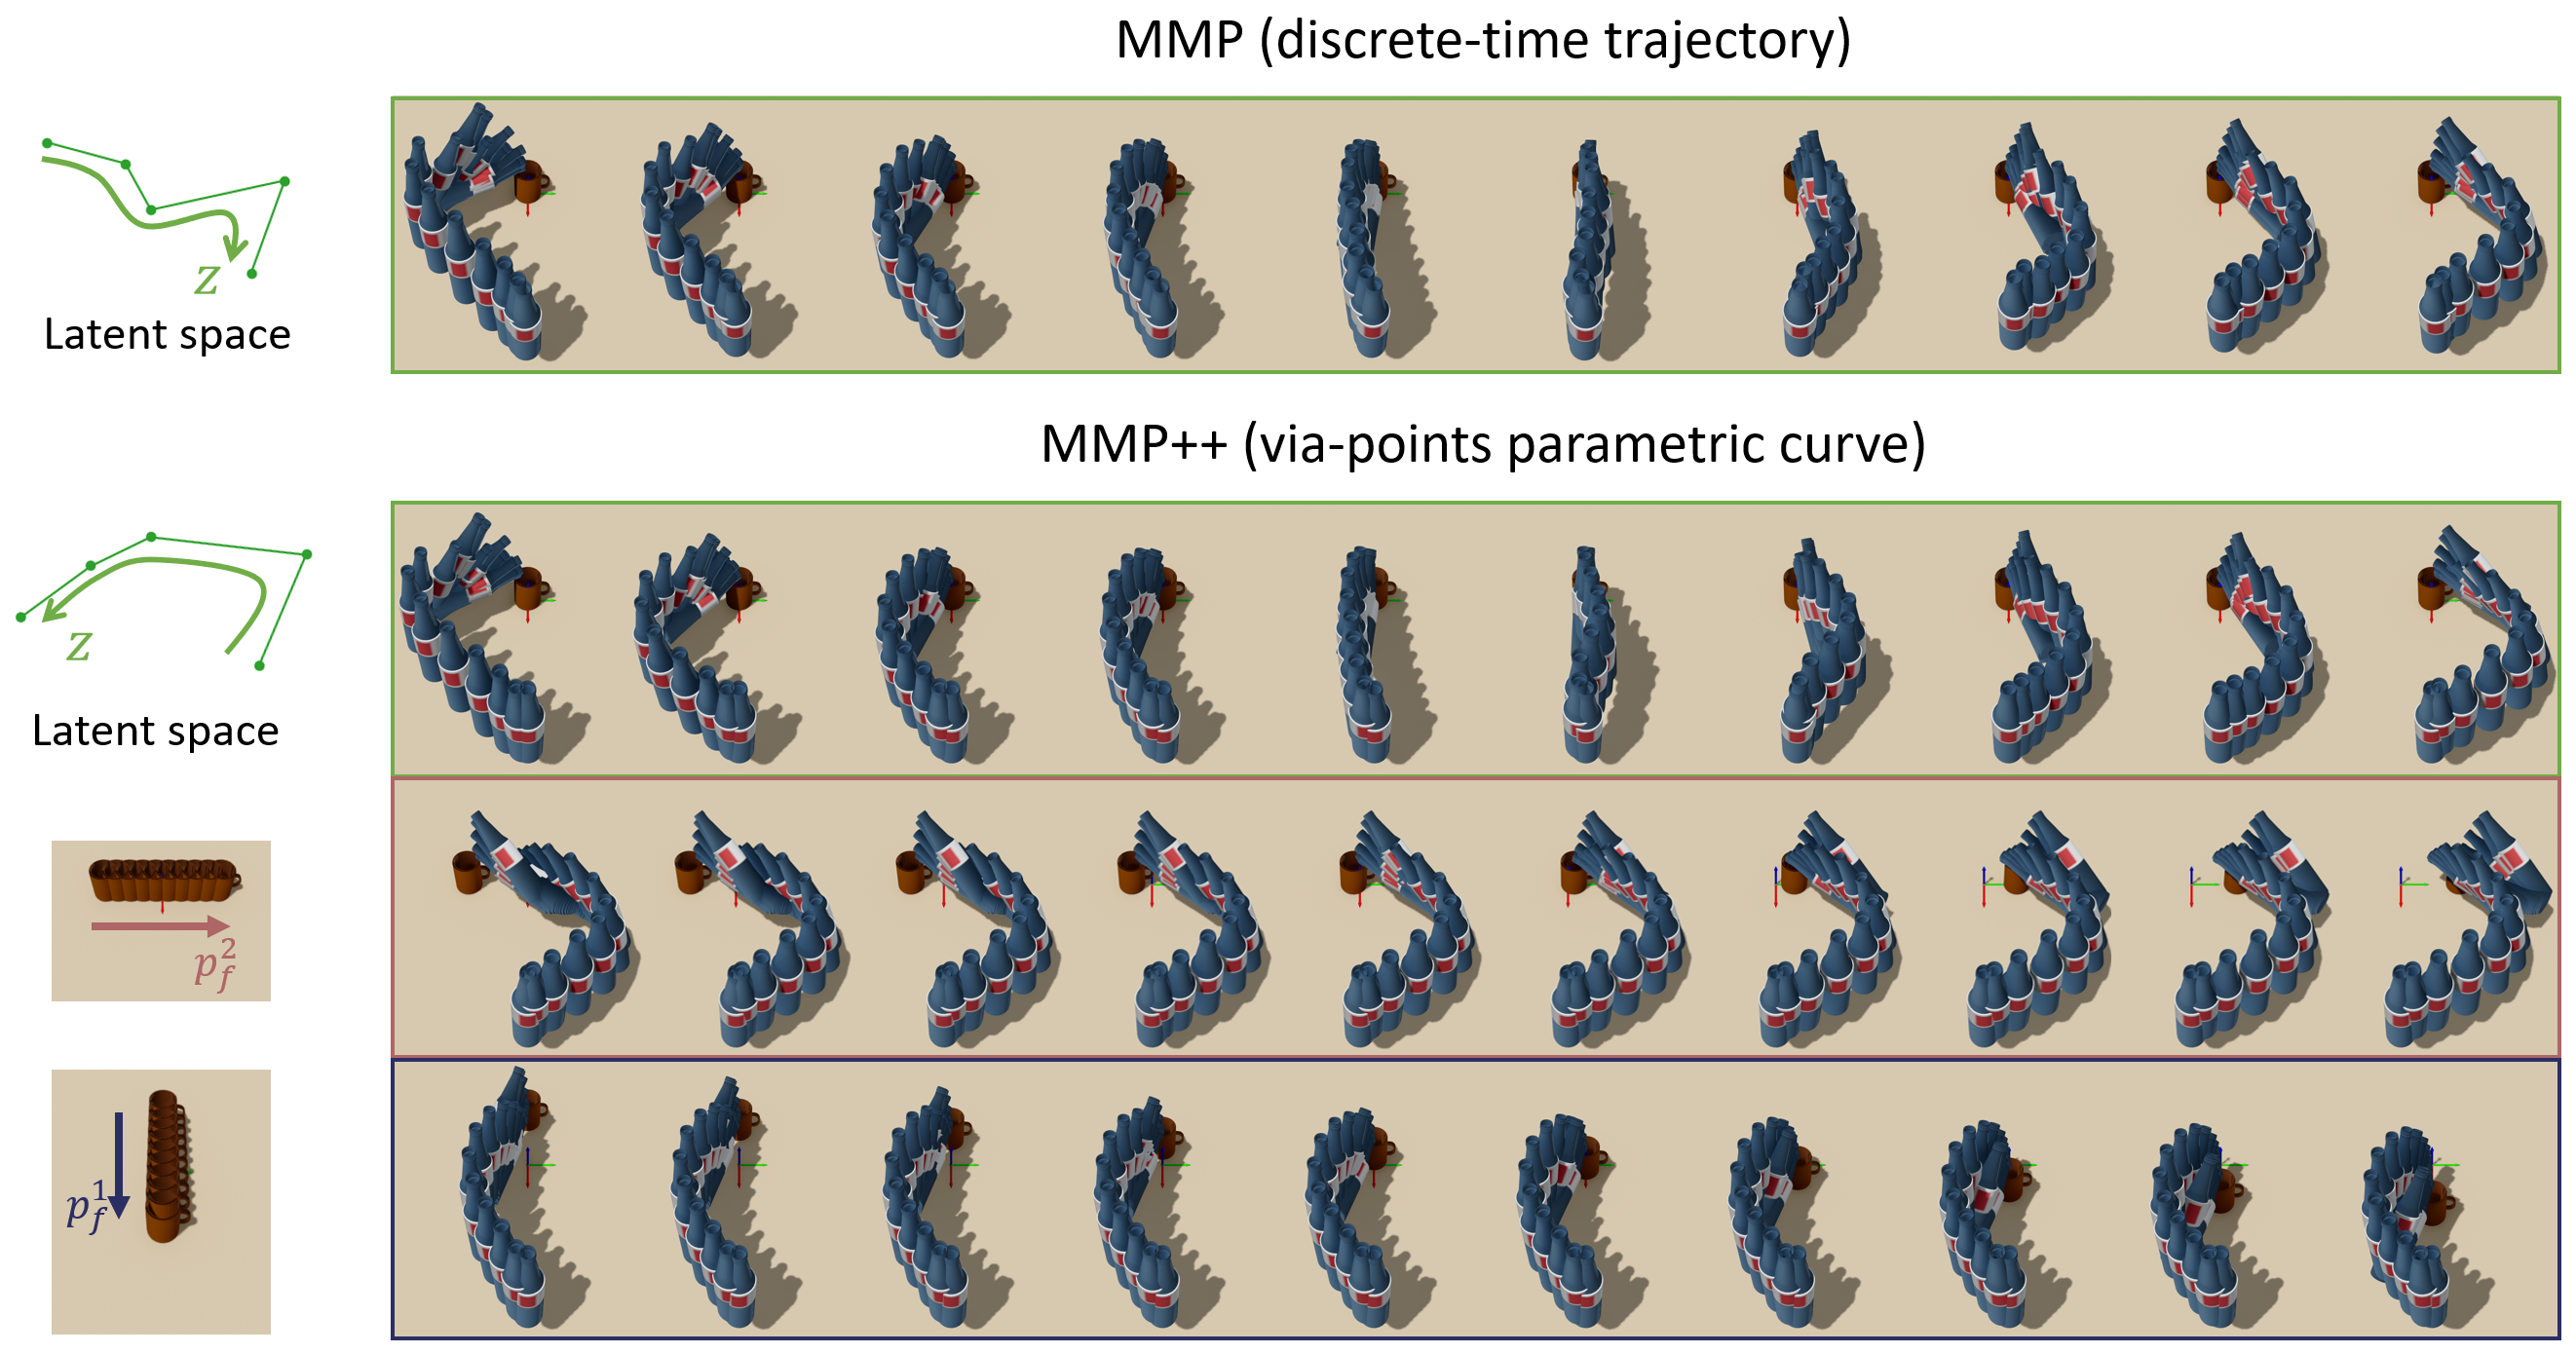
\includegraphics[width=0.85\textwidth]{figure/wp_results.png}
    \caption{The modulation of MMP trained to generate discrete-time trajectories and MMP++ trained to generate curve parameters of the trajectories. We can modulate latent values for both methods and generate smooth transitions of the SE(3) trajectories. In MMP++ ({\it Middle} and {\it Lower}), given continuous changes in the cup position, the water-pouring trajectories undergo smooth transitions.} 
    \label{fig:wp_results}
    \vspace{-5pt}
\end{figure*}

\begin{figure}[!t]
    \centering
    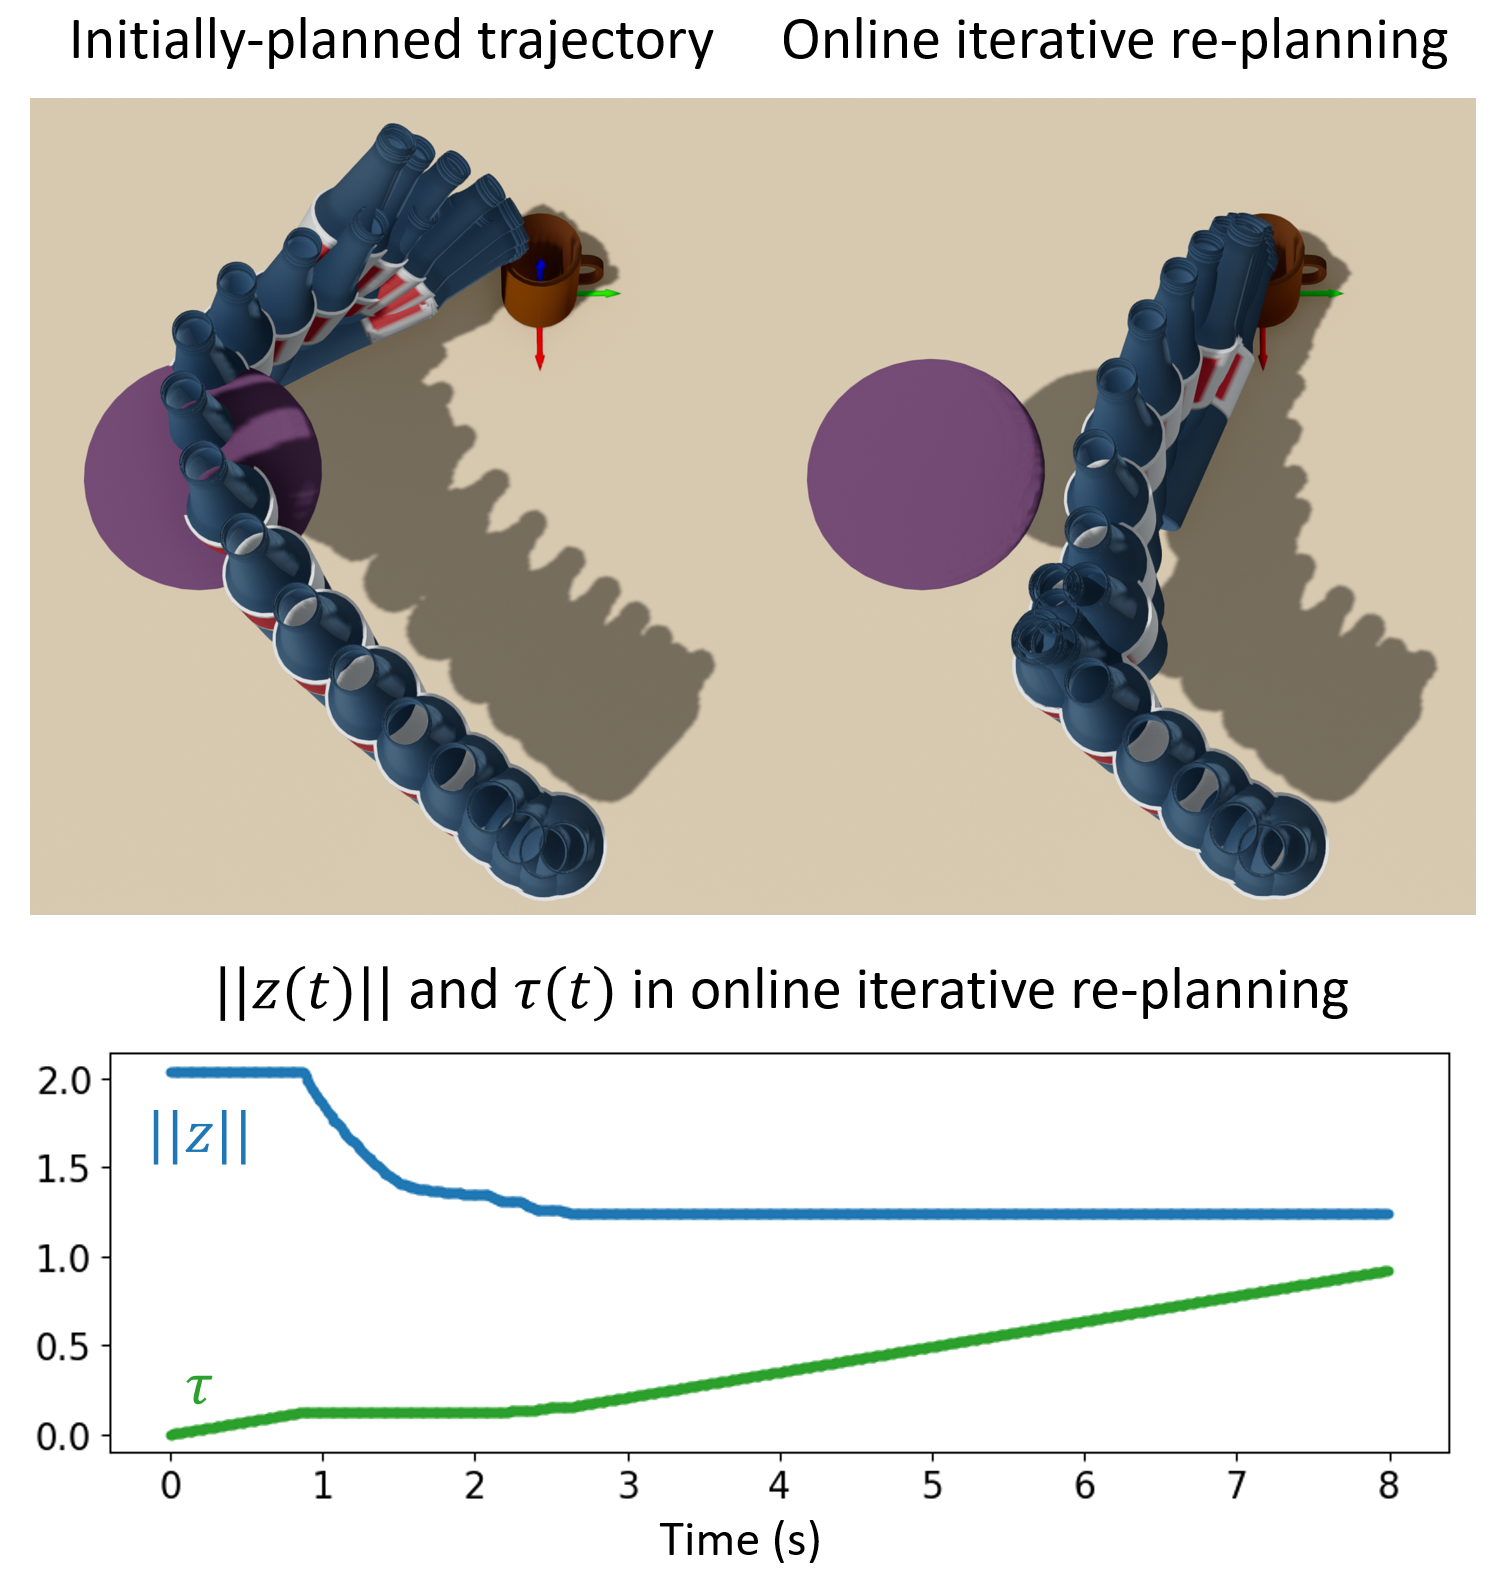
\includegraphics[width=0.9\linewidth]{figure/MPC2.png}
    \caption{{\it Upper-Left:} Initially-planned trajectory is blocked by the unseen obstacle during training. {\it Upper-Right:} We iteratively re-plan the bottle's SE(3) trajectory whenever it is predicted to collide with the obstacle. {\it Lower:} $\|z\|$ and $\tau$ as functions of time $t$ in online iterative re-planning ({\it Upper-Right}), where $T=7$, $t_w=0.2$, $f_c=100$, and $f_p=10$.} 
    \label{fig:MPC2}
    \vspace{-5pt}
\end{figure}

Consider the water-pouring SE(3) trajectory dataset in Fig.~\ref{fig:wp_dataset}. Our goal is to train an MMP++ with this dataset. 
First, note that the five trajectories in the dataset have the same initial SE(3) pose $(p_i, R_i)$ but have different final SE(3) poses $(p_f, R_f)$. Therefore, in addition to $(w_p, w_R)$, the final SE(3) pose $(p_f, R_f)$ is added to the curve parameter. To emphasize this, we denote the parametric curves by $p(\tau; w_p, p_f)$ and $R(\tau; w_R, R_f)$. Thus, our autoencoder $g,f$ is trained by using $\{(w_p, w_R, p_f, R_f)_i\}_{i=1}^{5}$ where each of these parameters is fitted to the demonstration trajectory. 

To construct neural network encoder and decoder, some cares need to be taken since $R_f\in{\rm SO}(3)$ is not a vector data. For the encoder $g: (w_p, w_R, p_f, R_f) \mapsto z$, we can flatten $R_f$ to a 9-dimensional vector and treat $(w_p, w_R, p_f, R_f)$ as a $6B+12$-dimensional vector input. For the decoder $f:z \mapsto (w_p, w_R, p_f, R_f)$, the orientation output $R_f$ should satisfy the rotation matrix constraints. To enforce this condition, we let $f:z \mapsto (w_p, w_R, p_f, w_f)$ where $w_f \in \mathbb{R}^{3}$ and map $w_f \mapsto \exp([w_f]) \in {\rm SO}(3)$.

For autoencoder training, we may use the L2 reconstruction loss in the parameter space $(w_p, w_R, p_f, R_f) \in \mathbb{R}^{6B + 12}$ as in (\ref{eq:recon_loss}). 
However, we found that this loss does not suitably capture the difference between the training and reconstructed SE(3) trajectories, resulting in an autoencoder with poor reconstruction qualities. Therefore, we use the following loss function: 
let $(\hat{w}_p, \hat{w}_R, \hat{p}_f, \hat{R}_f) = f\circ g(w_p,w_R,p_f,R_f)$ and $(p_\tau, R_\tau)$ be the SE(3) demonstration trajectory -- where $\tau$ denotes the normalized time parameter (i.e., for a total demonstration time length $T$, $\tau=t/T$) --, denoting the trajectory dataset by ${\cal D}=\{(p_\tau, R_\tau)_{i}\}_{i=1}^{5}$, the new reconstruction loss is    
\begin{align}
    \sum_{(p_\tau,R_\tau) \in {\cal D}} \int_{0}^{1} & \|p_\tau - p(\tau; \hat{w}_p, \hat{p}_f)\|^2  \nonumber \\ 
    & + \beta \| \log (R_\tau^T R(\tau; \hat{w}_R, \hat{R}_f)) \|_F^2 \: d\tau,
\end{align}
where $\beta>0$ and the integration over $\tau$ is approximately computed by the discrete sum.  

Fig.~\ref{fig:wp_results} shows the modulation results of the MMP trained with discrete-time trajectories as in~\cite{lee2023equivariant} and MMP++ with our parametric curve models. 
Both methods enable modulation of the latent value $z$, producing continuous transitions of water-pouring trajectories from left to right. 
Furthermore, MMP++ enables modulation of the initial and final poses $p_i,R_i,p_f,R_f$. As shown in Fig.~\ref{fig:wp_results} (MMP++: {\it Middle} and {\it Lower}), MMP++ produces pouring trajectories that adapt to changes in the cup position.

Lastly, we apply the online iterative re-planning algorithm using the water-pouring MMP++ in the presence of unseen obstacle. We use the re-planning algorithm in Algorithm~\ref{alg:OIR}. 
Similar to the robot arm experiment with the demo type 2 (manifold), we use the KDE density model (\ref{eq:KDE_density}). 
While the initially-planned SE(3) trajectory of the bottle collides with the purple spherical obstacle as shown in Fig.~\ref{fig:MPC2} ({\it Upper-Left}), the bottle's SE(3) trajectory is re-planned online when it is predicted to collide with the obstacle and successfully avoids the collision as shown in Fig.~\ref{fig:MPC2} ({\it Upper-Right}). Fig.~\ref{fig:MPC2} ({\it Lower}) shows $\|z\|$ and $\tau$ as functions of time, indicating when $(z,\tau)$ is re-planned. It can be confirmed that, from $t=1$ to $t=2.5$, collisions with the obstacle within the time interval $t_w=0.2$ are predicted and $(z, \tau)$ is re-planned multiple times. 


